% =====================================================================
% main.tex -- paper scaffold, content only, NOT compiled locally.
%
% *** READ BEFORE COMPILING OR SUBMITTING ***
%
% Preamble below was independently verified against the real template
% this session fetched directly: https://www.overleaf.com/latex/
% templates/formatting-instructions-for-neurips-2026/bjdwqfdkyftc
% (fetched and cross-checked twice on 2026-08-24). This is NOT a claim
% taken on trust from a supplied paste -- the previous paste for this
% same content (in an earlier request) contained real defects, found
% and fixed here rather than carried forward:
%   - `\usepackate{nicefrac}` -- typo for `\usepackage`; would fail to
%     compile ("Undefined control sequence").
%   - `\title{% TODO: ...}` with the TODO comment INSIDE the braces --
%     `%` consumes to end-of-line INCLUDING the newline, so this does
%     NOT leave the title blank; it silently sets `\title` to whatever
%     text sits on the following line before the closing brace. Fixed
%     below by moving the TODO to its own comment line above `\title{}`.
%   - The pasted author placeholder ("Anonymous Author(s) / Affiliation
%     / Address / email") does not match the real template's own
%     instructional placeholder ("David S.~Hippocampus, Dept. of
%     Computer Science, Cranberry-Lemon University, ..."). Kept
%     "Anonymous Author(s)" anyway, deliberately: that placeholder text
%     is the double-blind SUBMISSION convention overriding the
%     instructional demo text, not a template fact -- noted explicitly
%     here rather than conflated with the verified parts below.
%   - `\usepackage{natbib}` was NOT added as a separate line: the fetch
%     confirms `neurips_2026.sty` loads natbib itself; adding it again
%     risks a "package already loaded with different options" clash.
%   - `\usepackage{graphicx}` WAS added, even though it is not part of
%     the base template's own preamble (confirmed absent there) --
%     `paper/figures/` already holds Step 5's PDFs, so this paper will
%     need it regardless. Flagged here as an addition, not template
%     content.
%   - `\bibliographystyle{plainnat}` / `\bibliography{refs}` are not
%     shown verbatim in the template's own instructional body (which
%     only demonstrates manually-typeset example references) but are
%     the standard pairing given natbib is loaded -- kept as a
%     reasonable default, not claimed as literally template-verbatim.
%
% What is still NOT resolved, per this project's own explicit
% instruction not to fetch or fabricate it:
%   - The actual `neurips_2026.sty` class FILE this preamble depends on
%     to compile is still not present anywhere in this repository.
%     Compilation and page-count checks happen on Overleaf, where the
%     .sty is supplied by the official project/template sync, not here.
%   - `\input{checklist.tex}` (NeurIPS's mandatory paper checklist) is
%     confirmed required by the real template (present in the fetch
%     above) and is listed below, commented out with a TODO -- see the
%     note directly above that line. No placeholder checklist.tex has
%     been created: it is part of the same official author kit as the
%     .sty, subject to the same "don't fabricate it locally" rule, and
%     unlike a missing .sty, an incomplete or invented checklist would
%     misrepresent substantive answers (reproducibility, ethics,
%     broader impact) rather than just fail to compile.
% =====================================================================

\documentclass{article}

% Track/anonymity option -- confirmed valid: the real template lists
% `dblblindworkshop` among several commented-out track choices
% (alongside main, position, eandd, creativeai, sglblindworkshop,
% education). This project is a double-blind NewInML workshop
% submission via OpenReview, per the workshop's own CFP.
\usepackage[dblblindworkshop]{neurips_2026}

\usepackage[utf8]{inputenc}
\usepackage[T1]{fontenc}
\usepackage{hyperref}
\usepackage{url}
\usepackage{booktabs}
\usepackage{amsfonts}
\usepackage{nicefrac}
\usepackage{microtype}
\usepackage{xcolor}
\usepackage{graphicx} % added -- not in the base template, but this paper needs figures; see header note

\workshoptitle{New in ML at NeurIPS 2026}

% TODO: finalize title -- draft candidate recorded in SPEC.md's "Paper
% writing plan (Step 6.2)" section: "Isolating the Design Choice Behind
% NVFP4's Advantage over MXFP4". Not finalized; human decision.
\title{}

% Double-blind submission: anonymous author block. Real names/affiliations
% only at camera-ready, never before. Left empty pending that decision --
% not the template's own "David S.~Hippocampus" instructional placeholder,
% which is demo text for the formatting guide itself, not submission text.
\author{}

\begin{document}

\maketitle

\begin{abstract}
  % TODO -- written last, per the recommended writing order in SPEC.md's
  % "Paper writing plan (Step 6.2)" section.
\end{abstract}

% =====================================================
% Introduction — target length: TBD (no prior chat discussion
% establishing a target length or outline exists in this session or
% in this repository's tracked files/history — checked before writing
% this stub, not assumed; flagged rather than invented, see
% main.tex's header note).
% NOT YET WRITTEN.
% =====================================================

\section{Background}
\label{sec:background}

Both deployed FP4 formats store identical E2M1 elements (largest finite magnitude
6) and differ only in how a block is scaled (Table~\ref{tab:formats}).

\begin{table}[t]
  \centering
  \caption{The two block-scaled FP4 formats. Elements are identical; the scaling
    is the whole of the difference.}
  \label{tab:formats}
  \begin{tabular}{@{}l p{3.4cm} p{4.2cm}@{}}
    \toprule
                              & MXFP4                          & NVFP4 \\
    \midrule
    element format            & E2M1 (1/2/1)                    & E2M1 (1/2/1) \\
    block size                & 32                             & 16 \\
    block scale format        & E8M0 (0/8/0), a power of two    & E4M3 (1/4/3) \\
    global scale              & none                           & one per tensor (FP32) \\
    scale range               & $2^{-127}$ to $2^{127}$ (255 binades) & $2^{-9}$ to 448 relative to the global scale ($\sim$19 binades) \\
    scale resolution          & one binade (no mantissa bits)  & 6.25\% (3 mantissa bits) \\
    clipping of the block max  & impossible by construction     & up to $\sim$6\% \\
    specification / vendor    & OCP MX v1.0 \citep{ocp2023mx}   & NVIDIA \citep{nvidia2026nvfp4} \\
    \bottomrule
  \end{tabular}

  \vspace{0.6em}
  {\footnotesize Blocks run along the contraction axis. The MXFP4 block-scale
  exponent admits more than one rounding convention in the literature; the one
  used here is stated in Section~\ref{sec:method}. Scale-resolution and clipping
  figures follow from the format definitions, not derived here.}
\end{table}

The classical tools for this kind of product are the rounding-error bounds for an
inner product. For length $n$ and unit roundoff $u$, the deterministic worst case
is
$\gamma_n = n\,u/(1-n\,u)$ \citep{higham2002accuracy}, obtained by compounding one
rounding per accumulation step. A randomized analysis gives a more refined
estimate for typical cases, changing the leading factor to give a high-probability
bound of order $\sqrt{n \log n}\,u$ \citep{higham2019new}. Both are stated in
terms of a single unit roundoff $u$ fixed by the encoding.

NVIDIA's reported 36\%-more-tokens gap between the two formats
\citep{nvidia2026nvfp4} is given without an explanation of where the difference
comes from.

% =====================================================
% Method — target length ~1.5-2 pages, per SPEC.md's
% "Paper writing plan (Step 6.2) -- narrative structure".
%
% Every number, formula and design fact below is taken from
% SPEC.md, PREREGISTRATION.md, src/qgemm/bounds.py,
% src/qgemm/metrics.py and configs/sweep_main.yaml. No results
% are previewed here (Steps 4.1-4.4 belong to Section 4).
%
% Notation note: SPEC.md calls the derived bound `cota(n)`.
% Rendered here as \beta(n) -- an English-language paper should
% not carry the Spanish word untranslated. Same object, renamed
% only for the write-up.
%
% Base LaTeX math only (\[ \], equation, \frac, \sqrt, \mathrm):
% main.tex does not load amsmath, and this file deliberately does
% not require it.
% =====================================================

\section{Method}
\label{sec:method}

\subsection{Setup: backward error under exact accumulation}
\label{sec:method:setup}

The measurement instrument is a quantized GEMM. For operands $A \in
\mathbb{R}^{M \times n}$ and $B \in \mathbb{R}^{n \times N}$, both are quantized
with a block-scaled low-precision format along the contraction dimension $n$,
and the resulting float64 \emph{reconstructions} --- the dequantized values, not
the integer codes --- are multiplied. Accuracy is reported elementwise as the
backward error \citep{rasquinha2023metric}
\begin{equation}
  \mathrm{BE}_{ij} \;=\; \frac{\bigl|(AB)_{ij} - \hat{C}_{ij}\bigr|}
                              {\bigl(|A|\,|B|\bigr)_{ij}},
  \label{eq:be}
\end{equation}
with $\hat{C}$ the quantized product and $|\cdot|$ elementwise. The denominator
uses the product of absolute values, not $|AB|$; the two differ whenever the
exact product involves cancellation.

The primary route accumulates the reconstructions \emph{exactly}, in float64 ---
a design choice, not an implementation convenience. A low-precision GEMM has two
independent error sources, operands snapped onto a coarse grid and partial sums
rounded in a narrow accumulator, and they compose, so a number measured with
both active cannot be attributed to either. Under exact accumulation the only
remaining approximation is quantization of the inputs, so the residual
$\hat{C} - AB$ \emph{is} the input-quantization error and (\ref{eq:be}) isolates
it. A bfloat16 accumulator exists as a deliberate secondary ablation, outside
the grid analysed here and never mixed into a headline result.

Operands have i.i.d.\ t-Student($\nu$) entries --- smaller $\nu$ meaning heavier
tails, $\nu \to \infty$ the Gaussian case --- and each tensor is normalized as a
whole to unit median absolute deviation, rather than unit standard deviation,
which is undefined for the $\nu \le 2$ part of the grid. Every cell uses the
shape $(64,n) \times (n,64)$.

\subsection{Why the classical bound does not transfer}
\label{sec:method:classical}

The classical worst-case backward-error bound for a length-$n$ inner product is
$\gamma_n = nu/(1-nu)$ at unit roundoff $u$ \citep{higham2002accuracy};
probabilistic analyses relax the leading factor to $\sqrt{n}\,u$, or
$\sqrt{n \log n}\,u$ for a refined variant, as a high-probability upper bound
rather than a claim about typical growth
\citep{higham2019new,connolly2021stochastic}.

Neither transfers here, for a mechanistic reason. The $n$-dependence of both
families arises specifically from \emph{repeated rounding during accumulation}:
one rounding per summation step, $n$ of them, compounding either in the worst
case ($\gamma_n$) or as a random walk ($\sqrt{n}\,u$). Under exact accumulation
that mechanism is not physically present in the pipeline, so whatever
$n$-dependence the measured error has, it cannot be the one those bounds
describe. A block-scaled format also offers no fixed $u$ to substitute: the
classical unit roundoff is half an ulp of a grid fixed by the encoding, whereas
the grid an element lands on here is set by the largest magnitude in \emph{its
own block}, making the achieved relative error a distribution rather than a
property of the format.

\subsection{A measured unit roundoff, and the bound built from it}
\label{sec:method:bound}

The quantity replacing $u$ is measured directly. For a given element format,
block size, scale format and tail index $\nu$, define
\begin{equation}
  u_{\mathrm{eff}}(\mathrm{format}, \mathrm{block}, \nu)
  \;=\; \mathrm{median}_{\,i}\;
        \frac{\bigl|x_i - \hat{x}_i\bigr|}{\bigl|x_i\bigr|},
  \label{eq:ueff}
\end{equation}
the median per-element relative quantization error: draw samples from that
$\nu$, quantize under that configuration, read the median off the resulting
distribution. Its $99$th percentile is recorded alongside. Estimation uses an
independent calibration draw, seeded from a separate stream, so the denominator
of the ratio tested below is never calibrated on the sample it is tested against.

One choice inside (\ref{eq:ueff}) is load-bearing. Relative error is ill-defined
as $x_i \to 0$, and ``near zero'' means something only relative to an element's
own effective scale $s_{\mathrm{eff}}$ (block scale times global scale, where
one is used), since block scales span many orders of magnitude across a
heavy-tailed tensor. Elements with $|x_i| \le 0.25\,s_{\mathrm{eff}}$ are
therefore excluded. The threshold is not tuned: E2M1's smallest nonzero
magnitude is $0.5\,s_{\mathrm{eff}}$, so under round-to-nearest every element at
or below $0.25\,s_{\mathrm{eff}}$ quantizes to exactly zero with relative error
exactly $1$, recording the format's dynamic-range floor rather than its
precision. That the cut is necessary was checked, not assumed: with it disabled,
all $32$ measured configurations return $p_{99} = 1.00000$ exactly. Its price is
a large, configuration-dependent exclusion --- surviving fractions range from
$0.360$ (MXFP4 at $\nu=1$) to $0.932$ (NVFP4 at the Gaussian end) --- tabulated
wherever $u_{\mathrm{eff}}$ is reported.

Under exact accumulation the error at output entry $(i,j)$ is a sum of $n$
one-time input-quantization errors of essentially random sign, so partial
cancellation makes it grow like $\sqrt{n}$ rather than $n$, while the
denominator of (\ref{eq:be}), $\sum_k |A_{ik}|\,|B_{kj}|$, sums $n$ strictly
positive terms and grows approximately linearly for well-behaved inputs.
Together these give $\mathrm{BE} \sim \sqrt{n}\,u_{\mathrm{eff}}/n$, and hence
the tested bound
\begin{equation}
  \beta(n, \mathrm{format}, \mathrm{block}, \nu)
  \;=\; c \cdot
  \frac{u_{\mathrm{eff}}(\mathrm{format}, \mathrm{block}, \nu)}{\sqrt{n}},
  \label{eq:bound}
\end{equation}
which \emph{decays} in $n$ instead of growing. This is an order-of-magnitude
argument of the central-limit\slash law-of-large-numbers kind, not a proven
tight inequality, and is not offered as a theoretical contribution: both
premises --- a mean-zero numerator averaging like a random walk, a denominator
obeying a law of large numbers --- require moments the heaviest tails swept here
lack, and at $\nu=1$ (Cauchy) the derivation is expected to break down. That is
a limit of its assumptions, not a defect in the form of (\ref{eq:bound}).

The constant $c$ is fixed a priori at $c=1$ for all confirmatory analysis, per
the anti-circularity principle of this study's preregistration: a bound whose
constant is fitted to the same data it is tested against cannot be falsified by
that data. Keeping a unit leading constant follows the precedent of
probabilistic rounding analyses, which substitute $\sqrt{n}\,u$ for the
deterministic factor $nu$ without introducing a fitted constant
\citep{connolly2021stochastic}. Since the derivation is order-of-magnitude
rather than tight, a poorly calibrated $c=1$ is itself a reportable finding
rather than grounds to re-fit; any $\hat{c}$ estimated from data stays
descriptive and exploratory, never substituted back into the confirmatory ratio.

The bound is declared broken at $(\mathrm{format},\nu,n)$ when the lower end of
the $95\%$ bootstrap confidence interval of the median of $\mathrm{BE}/\beta(n)$
exceeds $1.0$: when error decays reliably more slowly than the cancellation rate
predicts, not when it exceeds a growing worst-case ceiling. Because
$u_{\mathrm{eff}}$ is itself indexed by $\nu$, both sides of the ratio move with
$\nu$, so this tests whether the \emph{scaling law} survives heavy tails, not
whether heavy tails increase absolute error.

\subsection{Factorial design}
\label{sec:method:design}

MXFP4 and NVFP4 differ in \emph{both} block size and scale format at once, so
any difference measured between the presets is unattributable --- block, scale
format, or interaction. The design crosses the two factors, block size $\in
\{16,32\}$ against scale format $\in \{\mathrm{E8M0},\mathrm{E4M3}\}$, so either
can be held fixed while the other varies; this $2 \times 2$ is the causal core.
The element format is E2M1 everywhere, since both real formats store E2M1 and
fixing it makes the scaling the only thing that varies. Use of a per-tensor
global scale is derived from the scale format rather than swept: E8M0 spans
$255$ binades and reaches any block's magnitude unaided, while E4M3 spans about
$19$ and overflows to NaN without one.

Two of the four combinations are real formats: block $32$ with an E8M0 scale is
MXFP4, block $16$ with an E4M3 scale is NVFP4. \textbf{The other two --- block
$16$ with E8M0, and block $32$ with E4M3 --- are experimental controls.} They
correspond to no hardware, no specification and no vendor format, and exist
solely as measurement instruments that make the comparison between the two real
formats separable. Nothing here proposes, endorses or benchmarks them as
formats, and results tables keep the distinction visible.

Rounding mode (round-to-nearest-even or stochastic) and a random Hadamard
transform (on or off) are secondary factors, not part of the causal core. The
transform is applied per block along the contraction dimension with the same
random signs on both operands, so it cancels inside every inner product and
needs no inversion, spreading a block's energy so a lone outlier no longer sets
the block scale. Per block by design: a global, whole-row transform spreads by
$\sqrt{n}$, tying its effect to the same $n$ whose scaling law this study sweeps.

These four factors are crossed with the tail index, which runs over
$\nu \in \{1,2,3,5,8,15,30\}$ together with the Gaussian limit, and with the
contraction dimension $n \in \{16,64,256,1024,4096\}$, for a grid of
$8 \times 5 \times 2^4 = 640$ cells, all with exact accumulation. The primary contraction
dimension is fixed in advance at $n=4096$, closest to real GEMM shapes in
language-model workloads; the other four are robustness checks, reported as a
disclosed sensitivity table and never substituted for it. Trial counts are
adaptive: $5000$ per cell at $\nu \in \{1,2,3\}$, where quantile estimates are
noisiest and the bound is most likely to break, and $1000$ per cell for the
lighter tails, for a total of $1.6$ million trials. Three per-tensor formats
(FP8-E4M3, FP8-E5M2 and INT8) are swept over the same $\nu$ grid at
$n \in \{16,256,4096\}$ as context baselines, outside the factorial and outside
every confirmatory comparison.

\subsection{Robust statistical protocol}
\label{sec:method:stats}

Each trial contributes a summary of its own $M \times N$ backward-error matrix,
and the \emph{trial} is the resampling unit throughout --- never the individual
matrix element, since elements within a block share a scale factor, are not
exchangeable, and would give anticonservative intervals that inflate the
measured break rate. Confidence intervals use the percentile bootstrap,
$B = 10{,}000$ resamples, an explicitly seeded generator, and are reported as
computed rather than forced symmetric.

The median and $90$th percentile carry all confirmatory statistical weight; the
$99$th percentile is reported for every cell but is indicative only, at any
trial count used here. The justification is a measured coverage gap, not a
generic warning that percentile bootstraps can be unreliable. A cell's $p_{99}$
is set by roughly its top $1\%$ of values ($10$ of $1000$ trials, $50$ of
$5000$), and a percentile bootstrap resamples with replacement from the observed
sample, so it can reweight those values but never produce one more extreme than
the largest already drawn. A coverage simulation quantifies this --- $1000$
simulated experiments per cell, t-Student($\nu=2$), both trial budgets, nominal
$95\%$: median coverage is $95.5\%$ at $1000$ trials and $94.8\%$ at $5000$,
close to nominal at both, while $p_{99}$ coverage is $92.7\%$ and $94.0\%$,
below the median's at both budgets and roughly $3.5$ standard errors below
nominal at $1000$ trials. The gap is real and directionally as the mechanism
predicts, but modest rather than a collapse; more trials measurably help
$p_{99}$ without closing it, which is why the indicative-only status holds at
every trial count rather than below some threshold.

\section{Results}
\label{sec:results}

\subsection{The Scaling Mechanism, Confirmed Where Its Assumptions Hold}
\label{sec:results:scaling}

``Confirmed'' and ``confirmatory'' here mean tested against a pre-fixed criterion
with $c$ pinned a priori, not a preregistered hypothesis that passed --- the
preregistered $\nu^\star$ hypothesis was undefined on this grid
(Section~\ref{sec:results:threshold}).

% n_scaling and nu_star share a width and are laid out as one physical two-up
% row -- two separately numbered captions in a single float. Figure 2
% (causal_heatmap, Sec. 4.2) is defined later; its number is reserved here by
% advancing the figure counter between the two captions below, and reclaimed at
% that later float. No \listoffigures, so nothing depends on the counter being
% monotone in source order.
\begin{figure}[t]
  \centering
  \begin{minipage}[t]{0.38\textwidth}
    \centering
    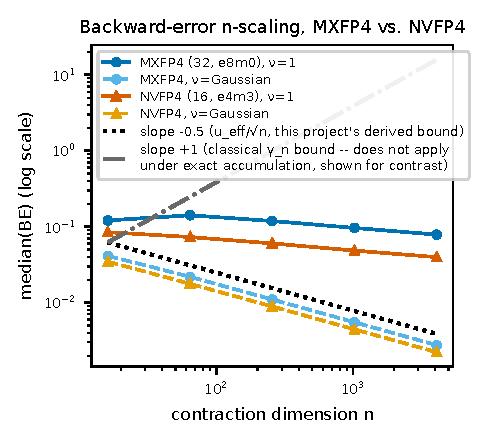
\includegraphics[width=\linewidth]{figures/figure2_n_scaling}
    \caption{Measured $\mathrm{median}(\mathrm{BE})$ against contraction length
      $n$ (log--log) for MXFP4 and NVFP4 at $\nu = 1$ and the Gaussian limit,
      against the obtained $u_{\mathrm{eff}}/\sqrt{n}$ slope $-0.5$ and the
      classical $\gamma_n$ slope $+1$ (shown for contrast, inapplicable under
      exact accumulation); the heavy tail decays far more slowly than $-0.5$.}
    \label{fig:n_scaling}
  \end{minipage}\hfill
  \begin{minipage}[t]{0.38\textwidth}
    \centering
    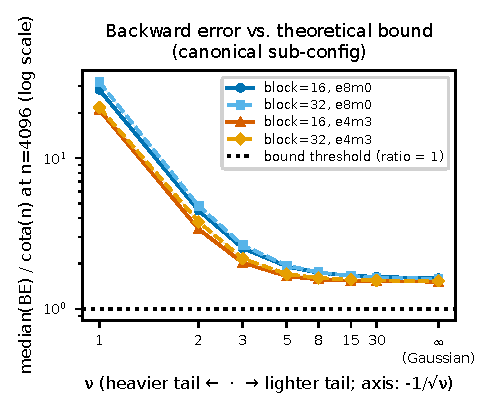
\includegraphics[width=\linewidth]{figures/figure1_nu_star}
    \addtocounter{figure}{1}% reserve Fig. 2 for the causal heatmap (Sec. 4.2)
    \caption{Median $\mathrm{BE}/\beta(n)$ at $n_{\mathrm{primary}} = 4096$
      versus tail index for all four block-size $\times$ scale-format arms;
      every curve sits above the ratio-$1$ threshold across the whole range, by
      roughly $20$--$32\times$ at $\nu = 1$ and $\sim$50--60\% at the Gaussian
      limit.}
    \label{fig:nu_star}
  \end{minipage}
\end{figure}

The empirical log--log slope of $\mathrm{median}(\mathrm{BE})$ against $n$ is
fitted by ordinary least squares for each of the 128 sub-configurations of the
sweep --- $8$ tail indices $\times$ $2$ block sizes $\times$ $2$ scale formats
$\times$ $2$ rounding modes $\times$ $2$ Hadamard settings --- over that
configuration's own 5 values of $n$, with a 95\% interval from 2000 bootstrap
replicates resampling each $n$'s trials independently. The reference is the
exponent $-0.5$ of (\ref{eq:bound}). Figure~\ref{fig:n_scaling} plots measured
$\mathrm{median}(\mathrm{BE})$ against $n$ for the two named presets; its
companion, Figure~\ref{fig:nu_star}, plots the same arms' error relative to the
bound $\beta(n)$ and is discussed in Section~\ref{sec:results:threshold}.

No configuration's interval contains $-0.5$; all 128 lie above it --- error
decays with $n$, but slower than the cancellation regime predicts, and nowhere
grows. That unanimity overstates the finding: it rests on a significance test
that at 1000--5000 trials excludes $-0.5$ even when the point estimate misses by
thousandths. By magnitude instead ($|\mathrm{slope} - (-0.5)| > 0.02$), 63 of 128
configurations deviate materially and 65 do not.

The split is ordered by tail weight, and the deviation shrinks smoothly and
monotonically as the tail lightens. At $\nu \in \{1, 2, 3\}$ every one of the 16
sub-configurations is material, with gaps from 0.041 to 0.490; the extreme is
$\nu = 1$, where the fitted slopes run from $-0.010$ to $-0.139$, one to two
orders of magnitude shallower than predicted rather than borderline. At
$\nu \in \{5, 8\}$ the sub-configurations straddle the threshold, some above and
some below, consistent with a smooth transition rather than a sharp cutoff. At
$\nu \in \{15, 30, \mathrm{Gaussian}\}$ none is material at any configuration, the
gap staying between 0.004 and 0.020.

The split follows the derivation's premises: the $-0.5$ exponent
(Section~\ref{sec:method:bound}) needs a mean-zero numerator behaving as a random
walk and a denominator obeying a law of large numbers --- moments the heaviest
tails lack ($\nu = 1$ is Cauchy). It is recovered to within 0.02 where those
moments exist and departs where they do not (Figure~\ref{fig:n_scaling}).

\subsection{Scale Format, Not Block Size, Is the Larger Lever}
\label{sec:results:decomposition}

The $2\times2$ design is read directly off the measured backward error, with no
theoretical bound involved. This partition is exploratory and post-hoc, adopted
under a dated preregistration amendment (Sec.\ 8.4) once the preregistered
$\nu^\star$ comparison (P1--P3) was left undefined by the finding of
Section~\ref{sec:results:threshold}. For each combination of tail
index, contraction dimension, rounding mode and Hadamard setting, three
statistics are formed in log space,
\[
\begin{array}{l}
  \mathrm{effect}_{\mathrm{block}} = \mathrm{median}(\log \mathrm{BE} \mid \mathrm{block}{=}16) - \mathrm{median}(\log \mathrm{BE} \mid \mathrm{block}{=}32) \\[3pt]
  \mathrm{effect}_{\mathrm{scale}} = \mathrm{median}(\log \mathrm{BE} \mid \mathrm{scale}{=}\mathrm{E4M3}) - \mathrm{median}(\log \mathrm{BE} \mid \mathrm{scale}{=}\mathrm{E8M0}) \\[3pt]
  \mathrm{interaction} = [\,(16,\mathrm{E4M3}) - (32,\mathrm{E4M3})\,] - [\,(16,\mathrm{E8M0}) - (32,\mathrm{E8M0})\,]
\end{array}
\]
each marginal effect aggregating over the other factor, with a 95\%
percentile-bootstrap interval from 2000 replicates resampling all four underlying
cells in one shared pass. Neither the tail index nor $n$ is collapsed.

Scale format moves the measured error more than block size does at every one of
the 40 canonical cells (8 $\nu$ $\times$ 5 $n$, round-to-nearest, no Hadamard
transform), and the ranking survives the secondary factors: scale format leads in
34 of 40 cells with the Hadamard transform on, 38 of 40 during stochastic
rounding, and 35 of 40 with both, never reversing to an overall block-size
majority in any of the four combinations. At $n = 4096$, canonically,
$\mathrm{effect}_{\mathrm{scale}}$ ranges from $-0.162$ at the Gaussian end to
$-0.389$ at $\nu = 2$, against $-0.042$ to $-0.246$ for
$\mathrm{effect}_{\mathrm{block}}$ (Figure~\ref{fig:causal_heatmap}): the
scale-format effect is about $3.9\times$ the block-size effect near the Gaussian
end, falling to roughly $2\times$ at $\nu = 2$ and about $1.1\times$ at
$\nu = 1$, where the two intervals still do not overlap (below). Both effects are negative at every
$n \ge 64$, so block $= 16$ and E4M3 --- NVFP4's two choices --- each reduce
measured error relative to their alternatives, and the larger of the two
reductions is the scale format.

The ranking is identical at all 5 values of $n$, at every $\nu$, with no crossing
anywhere in the grid, so the practical answer here --- unlike the threshold
analysis of Section~\ref{sec:results:threshold} --- does not depend on which $n$
had been designated primary. The $n = 16$ column is the apparent exception, and
it is not measuring block size at all: zero-padding leaves $\max|x|$ unchanged,
so a nominal block size of 32 spans the same 16 elements, with the same scale, as
block size 16 does. The effect first becomes measurable at $n = 64$, where the
two arms are genuinely different quantizers, and is essentially flat through
$n = 4096$ (at $\nu = 1$: $-0.286, -0.270, -0.257, -0.246$).

The margin $|\mathrm{effect}_{\mathrm{scale}}| - |\mathrm{effect}_{\mathrm{block}}|$
is thinnest at $\nu = 1$ (0.016 to 0.043 for $n \ge 64$) and wider on either side
--- 0.16 to 0.19 at $\nu = 2$, 0.124 to 0.135 at $\nu = 15$ --- but never
crosses: no point estimate flips at any of the 40 canonical cells, and at
$n = 4096$ the intervals are disjoint,
$|\mathrm{effect}_{\mathrm{block}}| \in [0.2395, 0.2510]$ against
$|\mathrm{effect}_{\mathrm{scale}}| \in [0.2719, 0.2831]$.

Backward error, not $u_{\mathrm{eff}}$, carries the headline comparison: it
determines GEMM output accuracy, whereas $u_{\mathrm{eff}}$
(Section~\ref{sec:method:bound}) is a per-element diagnostic. On $u_{\mathrm{eff}}$
the block-size effect leads at $\nu = 1$ and crosses the scale effect by
$\nu = 2$; in backward error the direction replicates but the crossing does not.
With the backward-error effects near parity for $\nu \le 2$, the clean ``scale
format dominates'' reading holds only at light-to-moderate tails, not the
heaviest ones that motivate the study.

The two factors are not purely additive: the interaction term is significant at
essentially every cell with $n \ge 64$, from $-0.095$ at $\nu = 1$ to $-0.028$ at
the Gaussian end at $n = 4096$. The dominance comparison above uses the pooled
marginal effects; at $\nu = 1$ the interaction is about a third of either main
effect, so that comparison is a simplification, not an exact partition.

\begin{figure}[t]
  \centering
  \addtocounter{figure}{-2}% reclaim the number reserved in the Sec. 4.1 two-up
  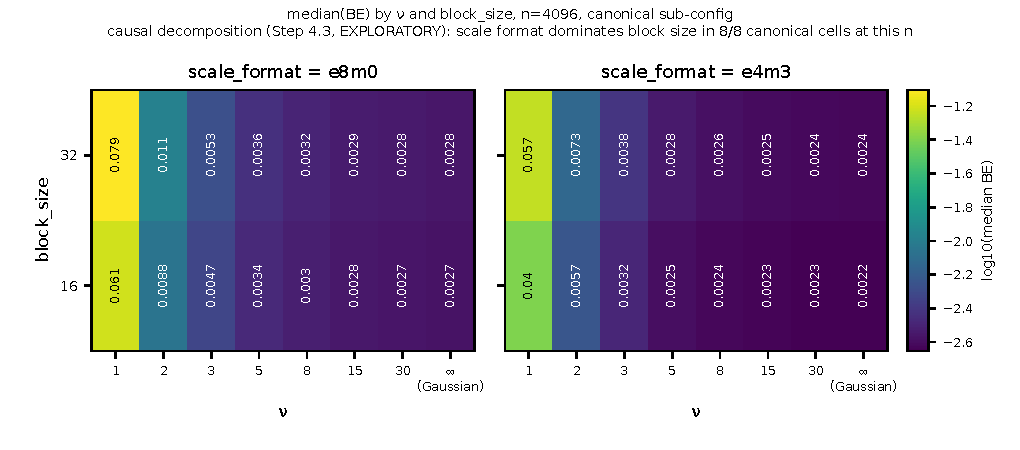
\includegraphics[width=0.66\textwidth]{figures/figure3_causal_heatmap}
  \caption{$\mathrm{median}(\mathrm{BE})$ over the block size $\times$ tail
    index grid at fixed $n = 4096$, split by scale format (E8M0 vs.\ E4M3);
    changing the scale format shifts the cells more than changing the block
    size at every $\nu$, though by a margin that narrows sharply toward the
    heaviest tail ($\nu = 1$).}
  \label{fig:causal_heatmap}
  \addtocounter{figure}{1}% restore counter past the two-up's Fig. 3
\end{figure}

\subsection{Why the Analysis Is Framed by Magnitude and Not by a Threshold}
\label{sec:results:threshold}

\looseness=-1 That decomposition replaced a preregistered plan: locate
$\nu^\star$, the tail index at which $\beta(n)$ first fails by the criterion of
Section~\ref{sec:method:bound}, for each of the 16 families, and compare the two
block sizes by where their $\nu^\star$ falls.

The bound is broken at every one of the 8 tested tail indices, in every one of
the 16 families, at $n_{\mathrm{primary}} = 4096$, and 0 of the 16 is
non-monotone, so $\nu^\star$ is not simply hard to locate but undefined
everywhere on this grid. For the two named presets, canonically, the median ratio
at $\nu = 1$ is 31.92 [31.85, 31.97] for MXFP4 and 20.91 [20.85, 20.97] for
NVFP4, against 1.588 [1.585, 1.590] and 1.515 [1.513, 1.517] at the Gaussian
limit. Even in the near-Gaussian regime, which the calculation's assumptions fit
best, the interval sits entirely above $1$: $c = 1$ under-predicts the measured
error by roughly 50 to 60\% there, and by a factor of 20 to 32 at $\nu = 1$
(Figure~\ref{fig:nu_star}).

This is not an artifact of the primary contraction dimension: the same pattern
holds at all 5 values of $n$, 16 of 16 families censored above and 0 below at
each. For MXFP4 at $\nu = 1$ the ratio is already 3.55 at $n = 16$ and rises
through 7.18, 12.10 and 19.62 to 31.92 at $n = 4096$, growing in line with the
shallower-than-$(-0.5)$ exponent of Section~\ref{sec:results:scaling} rather than
closing.

The preregistration anticipates this outcome: its all-cells-censored-above
contingency states the tail range was mis-specified, the hypothesis untestable on
such a grid, and the result to be reported as a grid mis-specification, not a
confirmation. It is equally not a null --- the rank comparison returns equal
fragility for the two block sizes only because every rank is pinned at the
ceiling, the signature of a saturated measurement. The two confirmatory results
therefore separate cleanly: the functional form of (\ref{eq:bound}) is well
supported at $\nu \ge 15$ (Section~\ref{sec:results:scaling}), while its leading
constant, fixed at $c = 1$ by the anti-circularity constraint of
Section~\ref{sec:method:bound}, is not calibrated anywhere in the tested range.

\looseness=-1 With no $\nu^\star$ to locate, block size and scale format could not
be compared through the bound at all --- both sides are censored past the edge of
what was measured. This is why Section~\ref{sec:results:decomposition} addresses
the same practical question directly from measured magnitudes, rather than
through the threshold criterion above.

\section{Validation with Real Activations}
\label{sec:validation}

The t-Student model underlying every result above was checked against the
activations a real network produces. GPT-2 small \citep{radford2019language} was
run over 300 non-empty lines of the WikiText-2 \citep{merity2016pointer} raw test
split, giving 34,390 valid tokens, and activations were captured at three of its
twelve transformer blocks --- h0, h6 and h11, the first, middle and last --- all
at the attention input projection (\texttt{attn.c\_attn}), so that depth is the
only thing varying across the three. Padded positions are removed before any
statistic or GEMM operand sees them. Tail weight is summarized by excess kurtosis
in Fisher's convention, in which a Gaussian is 0 and not 3, computed over the
full flattened tensor as a single distribution.

Each layer's excess kurtosis $k$ is mapped to an equivalent tail index through
$\nu = 4 + 6/k$, the closed-form inverse of a t-Student's $k = 6/(\nu - 4)$,
which is defined only for $\nu > 4$. The out-of-domain case is $k \le 0$, which
no t-Student attains and which the code reports as N/A with a stated reason
rather than extrapolating; it did not arise at any layer, though h6's
$\nu = 4.06$ sits within 0.06 of the boundary. The quantized-GEMM pipeline of
Section~\ref{sec:method:setup} is then run twice per layer and preset: once on
the real activations, once on a synthetic t-Student($\nu$) draw of identical
shape, rescaled so its median absolute deviation equals the real tensor's. The
layer's own weight matrix serves as operand $B$ in both arms, so the two runs
differ only in operand $A$'s tail shape.

Four of the six layer-preset cells land within 10\% of the t-Student prediction,
and none falls outside 50\%. At h0 (excess kurtosis 1.02, $\nu = 9.88$) and h11
(7.03, $\nu = 4.85$) the observed $\mathrm{median}(\mathrm{BE})$ equals the
predicted value to within 2--4\% under both presets: observed/predicted ratios of
0.997 and 0.987 at h0, 1.041 and 0.994 at h11. Layer h6 misses. Its excess
kurtosis is 101.9, two orders of magnitude beyond the other two layers, its
equivalent $\nu$ is 4.06, and its observed error runs 38\% (MXFP4) and 23\%
(NVFP4) \emph{higher} than predicted. The direction is the informative part: the
real activations produce \emph{more} backward error than a MAD- and
kurtosis-matched synthetic draw, so a single matched scalar under-describes how
concentrated h6's outlier mass is.

A targeted diagnostic on h6's own tensor, with no GEMM rerun, locates that
concentration. The twenty largest activation magnitudes in the entire
$34{,}390 \times 768$ tensor fall in exactly one channel, index 64, across twenty
distinct tokens. Within the top-1\% pool the same channel accounts for 13.0\% of
the mass and appears for all 34,390 tokens, the five most frequent channels for
58.2\%, and the top ten for 75.3\%; per-channel maxima drop sharply after a
handful (8.06, 7.08, 6.55, 5.31, then 2.76 for the next channel down). This is
the massive-activations pattern documented in transformer hidden states
\citep{sun2024massive}, and it violates an assumption the synthetic model makes
implicitly: that large values are randomly located and redrawn every sample,
where h6's are fixed to the same few channels on essentially every token. The
measured value also falls in a gap this study's own $\nu$-grid never samples:
$\nu \in \{1, 2, 3\}$ have undefined population excess kurtosis, outside the
closed form's $\nu > 4$ domain, while $\nu \ge 5$ tops out at 6 for the heaviest
finite-kurtosis grid point --- so 101.9 is finite but far past any value the grid
covers. Whether that structure mechanistically drives the 23--38\% gap, rather
than merely correlating with it, is not established here --- no ablation
separating channel structure from the kurtosis match was run, and none is
claimed.

This check is exploratory and bears on none of the confirmatory comparisons. It
tests the study's modeling choice, not any hypothesis about the formats, and
finds it sound across most of a real network --- failing only under extreme,
channel-concentrated kurtosis, where a single kurtosis-matched $\nu$ is
insufficient.

\section{Related Work and Limitations}
\label{sec:related}

This work builds directly on the backward-error methodology of
\citet{rasquinha2023metric}, extending it to block-scaled formats and
heavy-tailed operands. Two recent works approach FP4 microscaling from other
directions. \citet{fasoli2026finer} also measures block-size effects on model
correctness, but attributes degradation to \emph{narrow} tensor distributions ---
the opposite regime from the heavy tails swept here.
\citet{egiazarian2026bridging} analyses MXFP4 and NVFP4 error under a Laplace
operand model scored by per-element MSE, differing from this work in both metric
and operand model.

Six scope limits qualify these results. (i) The three per-tensor reference
formats --- FP8-E4M3, FP8-E5M2 and INT8 --- are in the frozen grid but never
executed, leaving MXFP4 and NVFP4 without a classical per-tensor baseline.
(ii) The random Hadamard transform is applied per block: a global, whole-row
transform would spread energy over $\sqrt{n}$, tying its effect to the same $n$
whose scaling law is under study, so global RHT is not evaluated here.
(iii) Quantization is CPU emulation in float64, not real quantized hardware.
(iv) Only E2M1 elements are studied. (v) Elements sharing a block share a
scale, so their errors are correlated rather than independent --- the leading
candidate behind the $u_{\mathrm{eff}}$ residual, consistent with a
survival-fraction gap whose rank order against the $u_{\mathrm{eff}}$ block-size
excess is perfect across all eight $\nu$ (Spearman 1.0), but not isolated by a
dedicated ablation. (vi) $c = 1$ is fixed a priori for
anti-circularity, so what is characterized is the bound's functional \emph{form},
not a calibrated absolute value.

\section{Conclusion}
\label{sec:conclusion}

Two design choices separate NVFP4 from MXFP4, and move this paper's
backward-error proxy unequally. Across the full grid of tail weights
and contraction lengths, the scale format moves the measured backward error more
than the block size does, at every canonical cell, and the ranking survives both
secondary factors --- stochastic rounding and the random Hadamard transform ---
without reversing anywhere. The margin narrows at the heaviest tail without
crossing. Whether that ordering carries over to training loss or the
token-efficiency gap is untested. This is a post-hoc
decomposition of measured magnitudes, not a preregistered test, and it involves
no theoretical bound at any point.

That last property is what the threshold analysis leaves behind. The constructed
bound breaks across the whole tested range, so the tail index at which it first
fails is undefined everywhere on this grid, and could not carry the planned
comparison; that null motivated the pivot to comparing magnitudes directly, and
does not bear on the decomposition, which never uses the bound. Two steps would
sharpen the picture: executing the specified but unrun per-tensor reference
cells, which would place both formats against a classical baseline, and an
ablation separating the intra-block correlation mechanism from other contributors
to the $u_{\mathrm{eff}}$ residual.


\begin{ack}
  % TODO -- funding/competing-interests disclosure, final version only.
\end{ack}

\bibliographystyle{plainnat}
\bibliography{refs}

% TODO: NeurIPS's mandatory paper checklist. The real template requires
% \input{checklist.tex} here. checklist.tex is part of the official
% author kit (same source/sync as neurips_2026.sty itself), is NOT
% present in this repository, and must NOT be fabricated locally --
% its answers (reproducibility, ethics, broader impact) are substantive,
% not boilerplate, so an invented or incomplete version would be worse
% than a visibly missing one. Pull it from the same Overleaf
% project/template sync that supplies the .sty, then uncomment:
% \input{checklist.tex}

\end{document}
